\documentclass[
  jou,
  floatsintext,
  longtable,
  a4paper,
  nolmodern,
  notxfonts,
  notimes,
  colorlinks=true,linkcolor=blue,citecolor=blue,urlcolor=blue]{apa7}

\usepackage{amsmath}
\usepackage{amssymb}



\usepackage[bidi=default]{babel}
\babelprovide[main,import]{spanish}
\StartBabelCommands{spanish}{captions} [unicode, fontenc=TU EU1 EU2, charset=utf8] \SetString{\keywordname}{Palabras
Claves}
\EndBabelCommands


% get rid of language-specific shorthands (see #6817):
\let\LanguageShortHands\languageshorthands
\def\languageshorthands#1{}

\RequirePackage{longtable}
\RequirePackage{threeparttablex}

\makeatletter
\renewcommand{\paragraph}{\@startsection{paragraph}{4}{\parindent}%
	{0\baselineskip \@plus 0.2ex \@minus 0.2ex}%
	{-.5em}%
	{\normalfont\normalsize\bfseries\typesectitle}}

\renewcommand{\subparagraph}[1]{\@startsection{subparagraph}{5}{0.5em}%
	{0\baselineskip \@plus 0.2ex \@minus 0.2ex}%
	{-\z@\relax}%
	{\normalfont\normalsize\bfseries\itshape\hspace{\parindent}{#1}\textit{\addperi}}{\relax}}
\makeatother




\usepackage{longtable, booktabs, multirow, multicol, colortbl, hhline, caption, array, float, xpatch}
\setcounter{topnumber}{2}
\setcounter{bottomnumber}{2}
\setcounter{totalnumber}{4}
\renewcommand{\topfraction}{0.85}
\renewcommand{\bottomfraction}{0.85}
\renewcommand{\textfraction}{0.15}
\renewcommand{\floatpagefraction}{0.7}

\usepackage{tcolorbox}
\tcbuselibrary{listings,theorems, breakable, skins}
\usepackage{fontawesome5}

\definecolor{quarto-callout-color}{HTML}{909090}
\definecolor{quarto-callout-note-color}{HTML}{0758E5}
\definecolor{quarto-callout-important-color}{HTML}{CC1914}
\definecolor{quarto-callout-warning-color}{HTML}{EB9113}
\definecolor{quarto-callout-tip-color}{HTML}{00A047}
\definecolor{quarto-callout-caution-color}{HTML}{FC5300}
\definecolor{quarto-callout-color-frame}{HTML}{ACACAC}
\definecolor{quarto-callout-note-color-frame}{HTML}{4582EC}
\definecolor{quarto-callout-important-color-frame}{HTML}{D9534F}
\definecolor{quarto-callout-warning-color-frame}{HTML}{F0AD4E}
\definecolor{quarto-callout-tip-color-frame}{HTML}{02B875}
\definecolor{quarto-callout-caution-color-frame}{HTML}{FD7E14}

%\newlength\Oldarrayrulewidth
%\newlength\Oldtabcolsep


\usepackage{hyperref}




\providecommand{\tightlist}{%
  \setlength{\itemsep}{0pt}\setlength{\parskip}{0pt}}
\usepackage{longtable,booktabs,array}
\usepackage{calc} % for calculating minipage widths
% Correct order of tables after \paragraph or \subparagraph
\usepackage{etoolbox}
\makeatletter
\patchcmd\longtable{\par}{\if@noskipsec\mbox{}\fi\par}{}{}
\makeatother
% Allow footnotes in longtable head/foot
\IfFileExists{footnotehyper.sty}{\usepackage{footnotehyper}}{\usepackage{footnote}}
\makesavenoteenv{longtable}

\usepackage{graphicx}
\makeatletter
\newsavebox\pandoc@box
\newcommand*\pandocbounded[1]{% scales image to fit in text height/width
  \sbox\pandoc@box{#1}%
  \Gscale@div\@tempa{\textheight}{\dimexpr\ht\pandoc@box+\dp\pandoc@box\relax}%
  \Gscale@div\@tempb{\linewidth}{\wd\pandoc@box}%
  \ifdim\@tempb\p@<\@tempa\p@\let\@tempa\@tempb\fi% select the smaller of both
  \ifdim\@tempa\p@<\p@\scalebox{\@tempa}{\usebox\pandoc@box}%
  \else\usebox{\pandoc@box}%
  \fi%
}
% Set default figure placement to htbp
\def\fps@figure{htbp}
\makeatother







\usepackage{newtx}

\defaultfontfeatures{Scale=MatchLowercase}
\defaultfontfeatures[\rmfamily]{Ligatures=TeX,Scale=1}





\title{Pautas para la Presentación del Informe de Investigación en
Economía: Guía para Estudiantes}


\shorttitle{Pautas Informe Económico}


\usepackage{etoolbox}



\ccoppy{\textcopyright~2023}



\author{Edison Achalma}



\affiliation{
{Escuela Profesional de Economía, Universidad Nacional de San Cristóbal
de Huamanga}}




\leftheader{Achalma}

\date{2023-06-03}


\abstract{This document provides guidelines for economics students on
how to present a research report. It covers the formulation of research
problems, hypothesis testing, studying economic relationships, and model
building. It suggests a structured approach including problem statement,
objectives, significance, theoretical considerations, hypotheses,
methodology, and data analysis. This guide aims to assist students in
conducting rigorous and relevant economic research by outlining key
components and steps to follow in the research process. }

\keywords{economic research, research methodology, hypothesis
testing, economic models, data analysis}

\authornote{\par{\addORCIDlink{Edison Achalma}{0000-0001-6996-3364}} 
\par{ }
\par{   El autor no tiene conflictos de interés que revelar.    Los
roles de autor se clasificaron utilizando la taxonomía de roles de
colaborador (CRediT; https://credit.niso.org/) de la siguiente
manera:  Edison Achalma:   conceptualización, redacción}
\par{La correspondencia relativa a este artículo debe dirigirse a Edison
Achalma, Email: \href{mailto:elmer.achalma.09@unsch.edu.pe}{elmer.achalma.09@unsch.edu.pe}}
}

\usepackage{pbalance} 
\usepackage{float}
\makeatletter
\let\oldtpt\ThreePartTable
\let\endoldtpt\endThreePartTable
\def\ThreePartTable{\@ifnextchar[\ThreePartTable@i \ThreePartTable@ii}
\def\ThreePartTable@i[#1]{\begin{figure}[!htbp]
\onecolumn
\begin{minipage}{0.5\textwidth}
\oldtpt[#1]
}
\def\ThreePartTable@ii{\begin{figure}[!htbp]
\onecolumn
\begin{minipage}{0.5\textwidth}
\oldtpt
}
\def\endThreePartTable{
\endoldtpt
\end{minipage}
\twocolumn
\end{figure}}
\makeatother


\makeatletter
\let\endoldlt\endlongtable		
\def\endlongtable{
\hline
\endoldlt}
\makeatother

\newenvironment{twocolumntable}% environment name
{% begin code
\begin{table*}[!htbp]%
\onecolumn%
}%
{%
\twocolumn%
\end{table*}%
}% end code

\urlstyle{same}



\makeatletter
\@ifpackageloaded{caption}{}{\usepackage{caption}}
\AtBeginDocument{%
\ifdefined\contentsname
  \renewcommand*\contentsname{Tabla de contenidos}
\else
  \newcommand\contentsname{Tabla de contenidos}
\fi
\ifdefined\listfigurename
  \renewcommand*\listfigurename{Listado de Figuras}
\else
  \newcommand\listfigurename{Listado de Figuras}
\fi
\ifdefined\listtablename
  \renewcommand*\listtablename{Listado de Tablas}
\else
  \newcommand\listtablename{Listado de Tablas}
\fi
\ifdefined\figurename
  \renewcommand*\figurename{Figura}
\else
  \newcommand\figurename{Figura}
\fi
\ifdefined\tablename
  \renewcommand*\tablename{Tabla}
\else
  \newcommand\tablename{Tabla}
\fi
}
\@ifpackageloaded{float}{}{\usepackage{float}}
\floatstyle{ruled}
\@ifundefined{c@chapter}{\newfloat{codelisting}{h}{lop}}{\newfloat{codelisting}{h}{lop}[chapter]}
\floatname{codelisting}{Listado}
\newcommand*\listoflistings{\listof{codelisting}{Listado de Listados}}
\makeatother
\makeatletter
\makeatother
\makeatletter
\@ifpackageloaded{caption}{}{\usepackage{caption}}
\@ifpackageloaded{subcaption}{}{\usepackage{subcaption}}
\makeatother
\makeatletter
\@ifpackageloaded{fontawesome5}{}{\usepackage{fontawesome5}}
\makeatother

% From https://tex.stackexchange.com/a/645996/211326
%%% apa7 doesn't want to add appendix section titles in the toc
%%% let's make it do it
\makeatletter
\xpatchcmd{\appendix}
  {\par}
  {\addcontentsline{toc}{section}{\@currentlabelname}\par}
  {}{}
\makeatother

%% Disable longtable counter
%% https://tex.stackexchange.com/a/248395/211326

\usepackage{etoolbox}

\makeatletter
\patchcmd{\LT@caption}
  {\bgroup}
  {\bgroup\global\LTpatch@captiontrue}
  {}{}
\patchcmd{\longtable}
  {\par}
  {\par\global\LTpatch@captionfalse}
  {}{}
\apptocmd{\endlongtable}
  {\ifLTpatch@caption\else\addtocounter{table}{-1}\fi}
  {}{}
\newif\ifLTpatch@caption
\makeatother

\begin{document}

\maketitle

\hypertarget{toc}{}
\tableofcontents
\newpage
\section[Introduction]{Pautas para la Presentación del Informe de
Investigación en Economía}

\setcounter{secnumdepth}{-\maxdimen} % remove section numbering

\setlength\LTleft{0pt}


\section{Introducción}\label{introducciuxf3n}

Al iniciar el semestre académico, es fundamental que los alumnos definan
de manera precisa el objetivo de su trabajo de investigación y evalúen
su relevancia, factibilidad y valor agregado. Se recomienda tomar estas
decisiones después de revisar la literatura básica y explorar la
disponibilidad de información estadística sobre el tema de
investigación.

La investigación económica abarca una amplia diversidad y depende de la
formación, capacidad y motivación del investigador. Algunos ejemplos de
tipos de investigación incluyen:

\begin{enumerate}
\def\labelenumi{\arabic{enumi}.}
\item
  Comprobación de hipótesis: En esta modalidad, el alumno presenta una
  hipótesis acerca de un fenómeno económico y busca comprobarla en su
  trabajo de investigación. Por ejemplo: ``En la economía peruana, el
  mecanismo de transmisión de la política monetaria no es el canal de la
  tasa de interés, sino el canal del crédito''.
\item
  Estudio de relaciones: Aquí, el alumno plantea el problema y se enfoca
  en determinar las relaciones entre variables económicas. Por ejemplo:
  ¿Cuál es la relación entre las exportaciones y el crecimiento
  económico en el Perú? ¿Cuáles son los determinantes del tipo de cambio
  real en el Perú?
\item
  Formulación de modelos: En esta modalidad, el alumno formula o
  reformula modelos para la economía peruana con el objetivo de explicar
  el comportamiento de variables económicas. Por ejemplo: Formulación de
  un modelo macroeconómico que explique la determinación de salarios,
  precios y empleo en el corto plazo.
\end{enumerate}

A continuación, se presenta una estructura sugerida para la presentación
del informe de investigación.

\textbf{I. Planteamiento del problema}

\begin{figure}

\caption{\label{fig-1}Imagen 1}

\centering{

\pandocbounded{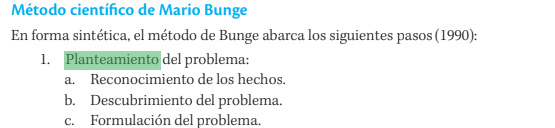
\includegraphics[keepaspectratio]{index_files/figure-html/20230603152205.png}}

}

\end{figure}%

En esta sección, el estudiante, después de revisar la bibliografía
relevante y los datos estadísticos relacionados con el problema
económico a estudiar, llevará a cabo:

Análisis cuantitativo y/o cualitativo del comportamiento de la variable
endógena (diagnóstico) - en este caso, el Producto Bruto Interno (PBI)
nacional, Impuesto Selectivo al Consumo (ISC), Impuesto General a las
Ventas (IGV), Impuesto a la Renta (IR) y otros impuestos.

Identificación de las causas del comportamiento de la variable endógena,
basado en la relación existente entre la variable endógena y la variable
exógena (explicación) - se puede emplear el método de Granger-MCO para
esto.

Exposición de propuestas de política económica basadas en la explicación
anterior (recomendación).

Formulación de preguntas que motiven respuestas en función del
diagnóstico, explicación y recomendación.

\textbf{II. Objetivos}

En esta sección, el estudiante debe presentar de manera clara sus
propósitos, tanto objetivos generales como específicos. Estos objetivos
deben formularse después de responder las siguientes preguntas:

\begin{enumerate}
\def\labelenumi{\arabic{enumi}.}
\tightlist
\item
  ¿Qué se desea lograr con la investigación?
\item
  ¿Qué conocimientos se busca adquirir?
\item
  ¿Qué se pretende demostrar?
\end{enumerate}

Es importante destacar que las respuestas a estas preguntas deben
contribuir a responder las interrogantes planteadas al final del
planteamiento del problema.

\textbf{III. Importancia y justificación}

En esta sección, el alumno expone las razones por las cuales plantea la
investigación. Estas motivaciones pueden tener un carácter teórico,
metodológico o práctico. Además, se pueden abordar las siguientes
interrogantes: \footnote{Para esta sección, resulta útil revisar Mendez
  (1995), páginas 92-97.}

\begin{itemize}
\tightlist
\item
  ¿Cuáles son los beneficios obtenidos al realizar esta investigación?
\item
  ¿Por qué resulta necesaria esta investigación?
\item
  ¿A quiénes beneficiará?
\item
  ¿Quiénes serán los potenciales usuarios?
\end{itemize}

\textbf{IV. Antecedentes}

En esta parte, el alumno debe revisar y presentar los trabajos de
investigación empírica relacionados con el tema. En general, es esencial
presentar una síntesis de dichos estudios, haciendo énfasis en los
objetivos, la metodología utilizada, las conclusiones y las
recomendaciones.

\textbf{V. Consideraciones teóricas}

En esta sección, el alumno debe presentar la literatura teórica
relevante al problema seleccionado.

\textbf{VI. Hipótesis}

En esta parte, el alumno, basándose en los elementos teóricos expuestos
anteriormente, plantea una proposición de causa (variable exógena) y
efecto (variable endógena). Cabe recordar que una hipótesis en modelos
estáticos se traduce en palabras a partir de los resultados de los
ejercicios de estática comparativa.

\textbf{VII. Metodología y datos}

En esta sección, el alumno:

\begin{enumerate}
\def\labelenumi{\arabic{enumi}.}
\tightlist
\item
  Identifica el método a utilizar.
\item
  Identifica el tipo de investigación a realizar.
\item
  Presenta las variables económicas identificadas empíricamente.
\item
  Señala las fuentes de información y/o la forma de recopilación de los
  datos.
\item
  Describe el proceso de procesamiento de la información.
\end{enumerate}

\textbf{VIII. Esquema}

En esta parte, el alumno presentará el esquema de la estructura del
trabajo de investigación por capítulos. En cada capítulo, es necesario
identificar los objetivos específicos correspondientes.

\textbf{IX. Desarrollo del esquema de investigación}

En esta sección, los alumnos, basándose en gráficos, tablas, técnicas
estadísticas y econométricas, obtienen conclusiones y plantean
recomendaciones en cada capítulo del esquema planteado.

\textbf{X. Bibliografía}

Aquí el alumno presenta la lista de obras consultadas que han servido
para fundamentar el planteamiento del problema, los antecedentes, el
marco teórico y las hipótesis.

\section{Bibliografía}\label{bibliografuxeda}

Méndez Álvarez, C. E. (1995). Metodología: guía para elaborar diseños de
investigación en ciencias económicas, contables y administrativas.
Buenos Aires, Argentina: McGraw-Hill.

Mendoza Bellido, W. E. (2007). Cómo investigan los economistas: Guía
para elaborar y desarrollar un proyecto de investigación. Fondo
Editorial, PUCP.

\section{Publicaciones Similares}\label{publicaciones-similares}

Si te interesó este artículo, te recomendamos que explores otros blogs y
recursos relacionados que pueden ampliar tus conocimientos. Aquí te dejo
algunas sugerencias:

\begin{enumerate}
\def\labelenumi{\arabic{enumi}.}
\tightlist
\item
  \href{https://achalmaedison.netlify.app/investigacion-metodologia/posts/2023-06-03-ideas-de-investigacion-para-economia/index.pdf}{\faIcon{file-pdf}}
  \href{https://achalmaedison.netlify.app/investigacion-metodologia/posts/2023-06-03-ideas-de-investigacion-para-economia}{Ideas
  De Investigacion Para Economia}
\item
  \href{https://achalmaedison.netlify.app/investigacion-metodologia/posts/2023-06-03-pautas-de-presentacion-del-informe-de-investigacion/index.pdf}{\faIcon{file-pdf}}
  \href{https://achalmaedison.netlify.app/investigacion-metodologia/posts/2023-06-03-pautas-de-presentacion-del-informe-de-investigacion}{Pautas
  De Presentacion Del Informe De Investigacion}
\item
  \href{https://achalmaedison.netlify.app/investigacion-metodologia/posts/2025-01-12-recursos-de-bibliografia-y-documentacion/index.pdf}{\faIcon{file-pdf}}
  \href{https://achalmaedison.netlify.app/investigacion-metodologia/posts/2025-01-12-recursos-de-bibliografia-y-documentacion}{Recursos
  De Bibliografia Y Documentacion}
\item
  \href{https://achalmaedison.netlify.app/investigacion-metodologia/posts/2025-02-09-recursos-para-traducción-y-correccion/index.pdf}{\faIcon{file-pdf}}
  \href{https://achalmaedison.netlify.app/investigacion-metodologia/posts/2025-02-09-recursos-para-traducción-y-correccion}{Recursos
  Para Traducción Y Correccion}
\end{enumerate}

Esperamos que encuentres estas publicaciones igualmente interesantes y
útiles. ¡Disfruta de la lectura!






\end{document}
